\chapter{Metodologia}

    Buscando inspiração nos projetos correlatos, bem como procurando se aproveitar dos benefícios de arquiteturas distribuídas. Foi construída uma arquitetura onde todas as entidades são independentes umas das outras, se comunicando através de um protocolo em comum. Sendo assim, torna-se possível escalar a capacidade de processamento de maneira horizontal, através da replicação de entidades específicas, atendendo maiores demandas de vazão do sistema. 

\section{Visão geral}

    \begin{figure}[!ht]
    	\centering
    	\caption{Visão simplificada da arquitetura implementada}
    
    	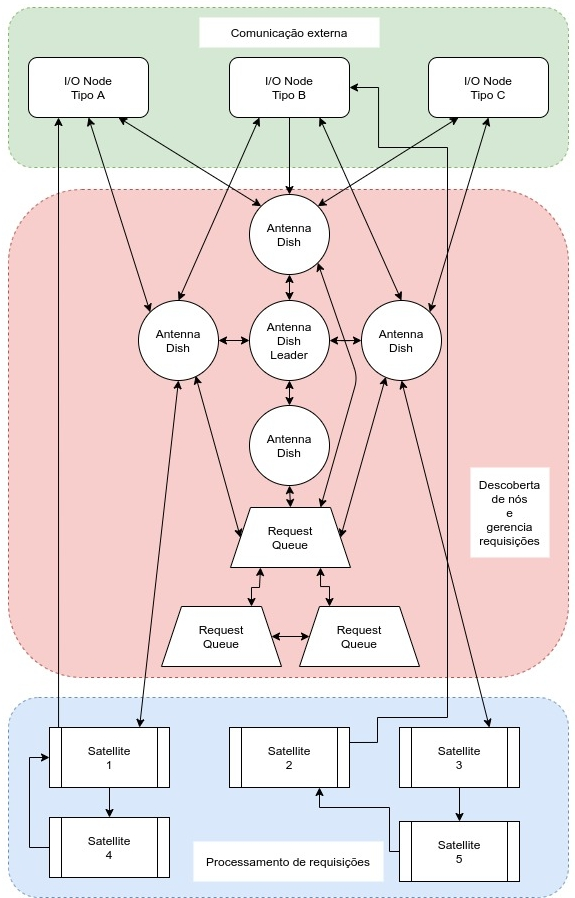
\includegraphics[width=12.5cm]{figuras/metodologia/antenna_simplified_diagram.jpg}
    	\legend{As três partes em que podemos dividir a arquitetura do sistema, as entidades da qual o sistema é composto e suas comunicações umas com as outras.}
    	\label{fig:antenna_simplified_diagram}
    \end{figure}

    Partindo da ideia de entidades independentes se comunicando, a arquitetura proposta, que pode ser conferida na figura \ref{fig:antenna_simplified_diagram}, pode ser dividida em três partes disjuntas. Estas partes representam a comunicação externa com os usuários do sistema, a descoberta de nós e gerência das requisições, bem como o processamento de fato das requisições.
    
    A partir do ponto de vista de um usuário, o único contato que ele consegue ter com o sistema é a camada externa. Esta camada é composta por entidades chamadas de \textit{"I/O Nodes"}, que são os responsáveis por receber os dados do cliente e devolver a resposta para o cliente quando estes dados tiverem sido processados. O conceito de tipos se dá para permitir que o sistema seja acessado por diversas fontes, tais como requisições HTTP ou por meio de escritas em banco de dados. Para o usuário, o restante do sistema é invisível, ele apenas envia suas requisições e algum tempo depois receberá a resposta.
    
    No lado oposto do sistema se encontram as entidades chamadas de \textit{"Satellites"}, responsáveis por processar os dados enviados pelos usuários. Nessa parte da arquitetura a ideia predominante é que cada um desses nós de processamento deve ser especializado numa única tarefa, de tal modo que processamentos complexos são feitos a partir de fluxos que passam por diversos nós. Ao fim do processamento, a resposta é enviada para um dos \textit{I/O Nodes}, que cuidará de transmitir a resposta para o usuário.
    
    Entre essas duas pontas existe uma camada de ligação, composta pelas entidades chamadas de \textit{"Antenna Dish"} e um sistema de fila distribuído. Nas \textit{Antenna Dish} são mantidos metadados sobre todo o sistema que são utilizados para a descoberta de nós. O sistema de fila distribuído é utilizado para enfileirar requisições em momentos de sobrecarga ou quando alguns dos serviços se encontra temporariamente indisponível.
    
    Todas as comunicações entre nós utiliza um protocolo de camada de aplicação próprio, desenvolvido sobre o protocolo de transporte QUIC. Uma vez que essa camada de transporte dispõe de características interessantes para o sistema, tais como cuidado com performance e segurança de comunicação. 

\section{Procotolo de comunicação}
    {\color{red} \# TODO: Detalhar sobre a escolha do QUIC e da framework de serialização}

\section{I/O Nodes}
    {\color{red} \# TODO: Detalhar sobre o funcionamento dos I/O Nodes e talvez falar sobre implementarmos a versão HTTP deles}

\section{Antenna Dish}
    {\color{red} \# TODO: Explicar sobre como é a estrutura distribuída das antennas dish, com subseções para o algoritmo de eleição}

\section{Request Queue}
    {\color{red} \# TODO: Explicar a escolha do sistema de filas utilizado e seu propósito}

\section{Satellites}
    {\color{red} \# TODO: Falar sobre o funcionamento dos satellites e do intercom, talvez enumerando possíveis aplicações por alto}